\section{Features}
In this section, we will highlight the main features of {\germinate}. This section will expand as we add new features.

\subsection{Internationalization and Localization}
\label{sec:features_i18n}
{\germinate} fully supports internationalization for an unlimited number of languages. Every text that you can see on the web interface can be localized. The language used on start-up is chosen based on the browser settings, but the user can easily switch to a different language by selecting it from the combo box at the bottom of the page. Have a look at Section \ref{sec:example_i18n} for usage details.

\subsection{News}
The {\germinate} web interface contains a place holder to show the latest news of the project. On the database side, these news are stored in two tables and can be updated at any time. The web interface will check the availability of news and show the three latest entries at the bottom of the page. Changes on the database side will immediately be visible on the website.

\subsection{Available pages}
\label{sec:pages}
This section gives an overview of all the pages that are available for {\germinate}. Based on your requirements and the data that is available, you can decide which pages should actually be available on the web interface and hide all others. The set of available pages can be changed dynamically without having to re-deploy the application. This gives you the freedom to customize your {\germinate} experience just as you please.

\subsubsection{About {\germinate}}
\begin{description}
	\item[Content]\hfill\\The about page of {\germinate} shows information about {\germinate} itself. This includes information about the developers and contact details.
	\item[Page name]\hfill\\\texttt{about-germinate}
	\item[Used data]\hfill\\None
\end{description}

\subsubsection{About Project}
\begin{description}
	\item[Content]\hfill\\This page shows information about the project itself.
	\item[Page name]\hfill\\\texttt{about-project}
	\item[Used data]\hfill\\None
	\item[Customization] You can change the content of this page by providing HTML to the \texttt{page.\allowbreak about.\allowbreak project.\allowbreak text} property.
\end{description}

\subsubsection{Accessions Overview}
\begin{description}
	\item[Content]\hfill\\The overview page shows all the accessions contained in the {\germinate} database in a filterable table. The user can sort, filter and mark items. Below the table, there are tools to download accessions, their attributes and pedigree data to flat files.
	\item[Page name]\hfill\\\texttt{accession-overview}
	\item[Used data]\hfill\\biologicalstatus, collectingsources, countries, germinatebase, institutions, locations, locationtypes, mlsstatus, pedigreedefinitions, pedigreedescriptions, pedigreenotations, pedigrees, storage, storagedata, subtaxa, synonyms, synonymtypes, taxonomies 
\end{description}

\subsubsection{Accessions for Collecting Site}
\begin{description}
	\item[Content] This page shows all accessions that have been collected at the given collecting site. It also allows the user to download the data in .kml format for Google Earth.
	\item[Page name]\hfill\\\texttt{accessions-for-collsite}
	\item[Used data]\hfill\\germinatebase, locations, locationtypes, countries
	\item[URL parameter]\hfill\\\texttt{collectingsiteId} The id of the collecting site.
\end{description}

\subsubsection{Acknowledgements}
\begin{description}
	\item[Content]\hfill\\This page can be used to acknowledge collaborators, etc.
	\item[Page name]\hfill\\\texttt{acknowledgements}
	\item[Used data]\hfill\\None
	\item[Customization] You can change the content of this page by providing HTML to the \texttt{page.\allowbreak acknowledgements.\allowbreak text} property.
\end{description}

\subsubsection{Administrator Configuration}
\begin{description}
	\item[Content]\hfill\\This page allows page administrators to make modifications to the way {\germinate} operates and looks. Regular users cannot see this page.
	\item[Page name]\hfill\\\texttt{admin-config}
	\item[Used data]\hfill\\None
\end{description}

\subsubsection{Allele Frequency Datasets}
\begin{description}
	\item[Content]\hfill\\All available allele frequency datasets are shown on this page. The user will be able to select which datasets to export.
	\item[Page name]\hfill\\\texttt{allele-freq-dataset}
	\item[Used data]\hfill\\allelefrequencydata, datasets, datasetstates, datasetpermissions, germinatebase, experiments, experimenttypes
\end{description}

\subsubsection{Allele Frequency Export}
\begin{description}
	\item[Content]\hfill\\On this page, the user is able to select which data they want to export from the selected dataset.
	\item[Page name]\hfill\\\texttt{allele-freq-export}
	\item[Used data]\hfill\\allelefrequencydata, datasets, datasetstates, datasetpermissions, germinatebase, experiments, experimenttypes, groupmembers, groups, maps, mapdefinitions, mapfeaturetypes, markers, markertypes
	\item[URL parameter]\hfill\\\texttt{allelefreqDatasetIds} The id of the allele frequency dataset. Single selection only.
\end{description}

\subsubsection{Allele Frequency Results}
\begin{description}
	\item[Content]\hfill\\On this page, the user can select the data binning scheme they want to apply to the allele frequency data. The final output files are shown on this page as well.
	\item[Page name]\hfill\\\texttt{allele-freq-results}
	\item[Used data]\hfill\\allelefrequencydata, datasets, datasetstates, datasetpermissions, germinatebase, experiments, experimenttypes, groupmembers, groups, grouptypes, maps, mapdefinitions, mapfeaturetypes, markers, markertypes
\end{description}

\subsubsection{Climate Data}
\begin{description}
	\item[Content]\hfill\\The climate data page shows detailed information about climate information. The data is visualized in charts and a color-coded table. In addition, climate data map overlays are shown on a map.
	\item[Page name]\hfill\\\texttt{climate-data}
	\item[Used data]\hfill\\climatedata, climateoverlays, climates, countries, datasets, datasetpermissions, datasetstates, experiments, experimenttypes, germinatebase, groupmembers, groups, grouptypes, locations, locationtypes, units
\end{description}

\subsubsection{Climate Datasets}
\begin{description}
	\item[Content]\hfill\\All available climate datasets are shown on this page. The user will be able to select which datasets to export.
	\item[Page name]\hfill\\\texttt{climate-dataset}
	\item[Used data]\hfill\\climatedata, climates, datasets, datasetstates, datasetpermissions, germinatebase, experiments, experimenttypes
\end{description}

\subsubsection{Chemical Compounds}
\begin{description}
	\item[Content]\hfill\\This page shows a table with all the chemical compounds.
	\item[Page name]\hfill\\\texttt{compound-details}
	\item[Used data]\hfill\\analysismethod, compounddata, compounds, datasets, germinatebase, units
\end{description}

\subsubsection{Chemical Compound Details}
\begin{description}
	\item[Content]\hfill\\The chemical compound details page shows information about a specific compound. This includes the compound data values across all accessions and visible datasets as well as that same data in the form of a chart. If images and external links are associated with a compound, these will be shown as well.
	\item[Page name]\hfill\\\texttt{compound-details}
	\item[Used data]\hfill\\analysismethod, compounddata, compounds, datasets, germinatebase, synonyms, synonymtypes, units
	\item[URL parameter]\hfill\\\texttt{compoundId} The id of the chemical compound.
\end{description}

\subsubsection{Chemical Compound Datasets}
\begin{description}
	\item[Content]\hfill\\All available chemical compound datasets are shown on this page. The user will be able to select which datasets to export.
	\item[Page name]\hfill\\\texttt{compound-dataset}
	\item[Used data]\hfill\\compounddata, compounds, datasets, datasetstates, datasetpermissions, germinatebase, experiments, experimenttypes
\end{description}

\subsubsection{Chemical Compound Data}
\begin{description}
	\item[Content]\hfill\\This page offers various different visualizations for the chemical compound data of the selected datasets. The data can also be downloaded into flat files.
	\item[Page name]\hfill\\\texttt{compound-data}
	\item[Used data]\hfill\\analysismethod, compounddata, compounds, datasets, germinatebase, synonyms, synonymtypes, units
	\item[URL parameter]\hfill\\\texttt{compoundDatasetIds} The ids of the chemical compound dataset.
\end{description}

\subsubsection{Cookie}
\begin{description}
	\item[Content]\hfill\\EU law requires us to provide information about the cookies that {\germinate} uses and what we use this information for. Detailed information about our usage of cookies is available on this page.
	\item[Page name]\hfill\\\texttt{cookie}
	\item[Used data]\hfill\\None
\end{description}

\subsubsection{Data Statistics}
\begin{description}
	\item[Content]\hfill\\The data statistics page visualizes aggregated information about the data contained in {\germinate}.
	\item[Page name]\hfill\\\texttt{data-stats}
	\item[Used data]\hfill\\Everything
\end{description}

\subsubsection{Dataset Overview}
\begin{description}
	\item[Content]\hfill\\This page shows all the datasets within {\germinate} independent of their type in one table.
	\item[Page name]\hfill\\\texttt{dataset-overview}
	\item[Used data]\hfill\\allelefrequencydata, climatedata, climates, compounddata, compounds, datasets, datasetstates, datasetpermissions, germinatebase, experiments, experimenttypes, phenotypedata, phenotypes, units
\end{description}

\subsubsection{Experiment Details}
\begin{description}
	\item[Content]\hfill\\The experiment details page shows all the datasets contained in a single experiment.
	\item[Page name]\hfill\\\texttt{experiment-details}
	\item[Used data]\hfill\\datasets, datasetpermissions, datasetstates, experiments, experimenttypes
	\item[URL parameter]\hfill\\experimentId The id of the experiment.
\end{description}

\subsubsection{Genotype Datasets}
\begin{description}
	\item[Content]\hfill\\All available genotype datasets are shown on this page. The user will be able to select which datasets to export.
	\item[Page name]\hfill\\\texttt{genotype-dataset}
	\item[Used data]\hfill\\datasets, datasetstates, datasetpermissions, germinatebase, experiments, experimenttypes
\end{description}

\subsubsection{Genotype Export}
\begin{description}
	\item[Content]\hfill\\On this page, the user is able to select which data they want to export from the selected dataset.
	\item[Page name]\hfill\\\texttt{genotype-export}
	\item[Used data]\hfill\\datasets, datasetstates, datasetpermissions, germinatebase, experiments, experimenttypes, groupmembers, groups, maps, mapdefinitions, mapfeaturetypes, markers, markertypes
	\item[URL parameter]\hfill\\\texttt{genotypeDatasetIds} The id of the genotype dataset. Single selection only.
\end{description}

\subsubsection{Geographic Search}
\begin{description}
	\item[Content]\hfill\\The geographic search page allows the user to search for both accessions and locations based on a given query point or polygon.
	\item[Page name]\hfill\\\texttt{geographic-search}
	\item[Used data]\hfill\\countries, germinatebase, locations, locationtypes
\end{description}

\subsubsection{Group Preview}
\begin{description}
	\item[Content]\hfill\\ {\germinate} offers the functionality to define groups of accessions via an API and a dedicated page. Tools like CurlyWhirly can upload a file containing the identifier of accessions and {\germinate} will display a preview of these items in a table. Once the user is happy with the selection, they can create a new group based on the selection.
	\item[Page name]\hfill\\\texttt{group-preview}
	\item[Used data]\hfill\\germinatebase, groupmembers, groups, grouptypes
\end{description}

\subsubsection{Groups}
\begin{description}
	\item[Content]\hfill\\The groups page shows an overview of all the accession, marker and location groups that are defined in {\germinate}. Depending on the permissions, the user can create new groups, delete old groups and modify the members of a group.
	\item[Page name]\hfill\\\texttt{groups}
	\item[Used data]\hfill\\countries, germinatebase, groupmembers, groups, grouptypes, locations, locationtypes, markers, markertypes
	\item[URL parameter]\hfill\\\texttt{groupId} The id of the group.
\end{description}

\subsubsection{Image Gallery}
\begin{description}
	\item[Content]\hfill\\This page shows all the images that are defined grouped by type. By clicking on the button below each image the user will be able to navigate to the corresponding details page.
	\item[Page name]\hfil\\\texttt{image-gallery}
	\item[Used data]\hfill\\compounds, germinatebase, images, imagetypes
	\item[URL parameter]\hfill\\\texttt{latitude}, \texttt{longitude} The location of the point query.
\end{description}

\subsubsection{Locations}
\begin{description}
	\item[Content]\hfill\\The locations page shows information about the location data. The locations are displayed on maps as well as visualized in different ways.
	\item[Page name]\hfill\\\texttt{locations}
	\item[Used data]\hfill\\countries, germinatebase, locations, locationtypes
\end{description}

\subsubsection{Home}
\begin{description}
	\item[Content]\hfill\\The home page of {\germinate}. It shows aggregated statistics about accessions, groups, locations and markers.
	\item[Page name]\hfill\\\texttt{home}
	\item[Used data]\hfill\\countries, germinatebase, groupmembers, groups, grouptypes, locations, locationtypes, markers, markertypes
\end{description}

\subsubsection{Institutions}
\begin{description}
	\item[Content]\hfill\\This page shows all the institutions associated with accessions held in {\germinate}.
	\item[Page name]\hfill\\\texttt{institutions}
	\item[Used data]\hfill\\countries, germinatebsae, institutions, locations, locationtypes
\end{description}

\subsubsection{Maps}
\begin{description}
	\item[Content]\hfill\\The maps page shows an overview of all the maps. Selecting one of them will display a table of all the markers on this map along with their position on the chromosome.
	\item[Page name]\hfill\\\texttt{maps}
	\item[Used data]\hfill\\mapdefinitions, mapfeaturetypes, maps, markers, markertypes
	\item[URL parameter]\hfill\\\texttt{mapId} The id of a map. This will expand the details of this map.
\end{description}

\subsubsection{Marked Items}
\begin{description}
	\item[Content]\hfill\\Marked item lists are a way of keeping track of items of interest. These items can be any accessions, markers or locations that the user is interested in. The marked items page shows all the items a user has marked so far. There are options to download the data or to create a group from the list if the user has sufficient permissions.
	\item[Page name]\hfill\\\texttt{marked-items}
	\item[Used data]\hfill\\germinatebase, groupmembers, groups, grouptypes, markers, markertypes, locations, locationtypes
\end{description}

\subsubsection{Marker Details}
\begin{description}
	\item[Content]\hfill\\This page displays information about a single marker. It shows which datasets the marker is part of as well as which maps it is on. Additionally, a list of all known synonyms is shown.
	\item[Page name]\hfill\\\texttt{marker-details}
	\item[Used data]\hfill\\mapdefinitions, mapfeaturetypes, maps, markers, markertypes, synonyms, synonymtypes
	\item[URL parameter]\hfill\\\texttt{markerId} The id of the marker.
\end{description}

\subsubsection{Mega Environments}
\todo{TODO}

\subsubsection{News}
\begin{description}
	\item[Content]\hfill\\This page shows news about {\germinate} and the contained data. The news items are sorted by creation date, so the latest one is shown first.
	\item[Page name]\hfill\\\texttt{news}
	\item[Used data]\hfill\\news, newstypes
\end{description}


\subsection{User registration}
\label{sec:registration}

{\germinate} can be used with and without authentication. This means that you can decide if you want to restrict access to your {\germinate} instance to registered users. If you decide to do so, you'll need people to be able to register. The registration form of {\germinate} (Figure \ref{fig:user_registration_registration}) provides a concise and easy way to register. If you choose to use a disclaimer that potential new users have to accept, this will appear before the form is visible. Once the user completes the form, they will either get access right away or you need to approve the new users manually. This is based on the setting of the property \texttt{Gatekeeper.Registration.Needs.Approval} (see Section \ref{sec:config-properties} for help). If you choose to use the approval approach, you'll see the screen shown in Figure \ref{fig:user_registration_approval} after selecting "Approve users" in Gatekeeper. The user will be notified with your decision.

\begin{figure}
    \centering
    \begin{subfigure}[b]{0.475\textwidth}
        \centering
        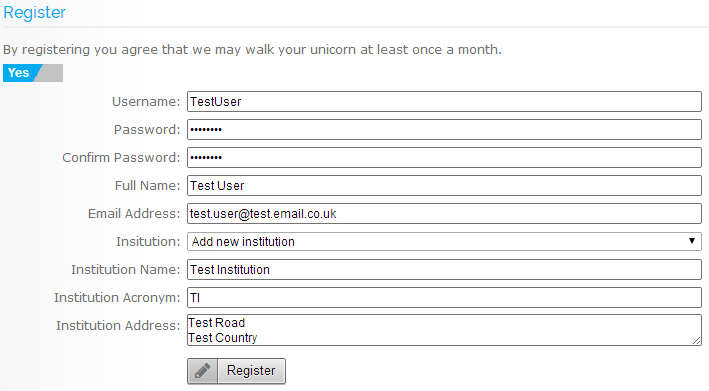
\includegraphics[width=1.0\textwidth]{img/features/registration.png}
        \caption{Registration form on the {\germinate} site}
        \label{fig:user_registration_registration}
    \end{subfigure}
    \hspace*{0.5cm}
    \begin{subfigure}[b]{0.475\textwidth}
        \centering
        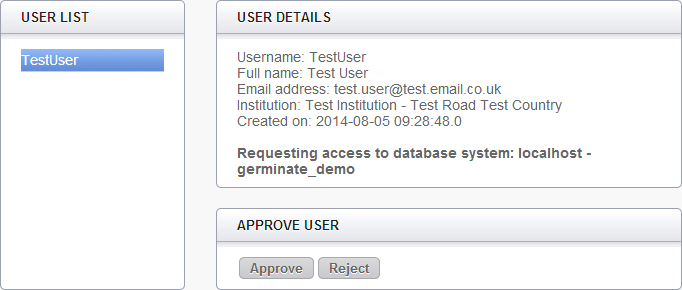
\includegraphics[width=1.0\textwidth]{img/features/registration-approve.png}
        \caption{Approval page on the Gatekeeper page}
        \label{fig:user_registration_approval}
    \end{subfigure}
    \caption{User registration}
    \label{fig:user_registration}
\end{figure}

\subsection{Groups}
{\germinate} allows you to define groupings of various items which makes exporting or visualizing data more comfortable. An intuitive example of groups are accession groups. A group of accessions can contain accessions that are similar to each other or a list of accessions that you want to export against a map for visualization in Flapjack.

A new group can be created with a couple of clicks: First, select the type of group that you want to create, \eg accession group, collecting site group, marker group etc. Afterwards, create a new group by just entering the name of the new group.

To delete group members, just select the group that you want to modify and check the items to remove in the table. Afterwards click on the delete button below the table. To delete a complete group, click on the delete icon next to the group selection box.

\subsection{Security}
\label{sec:example_security}
As already mentioned earlier, {\germinate} is equipped with a secure login system\footnote{{\germinate} is only as secure as the connection between client and server. Use a secure connection (TLS/SSL) to prevent password snooping.}. This feature is completely optional, but it allows you to protect your data from any unauthorized access. In this section, we will explain how the security system works and we will show what is necessary to use it properly.

\begin{figure}[h]
    \centering
    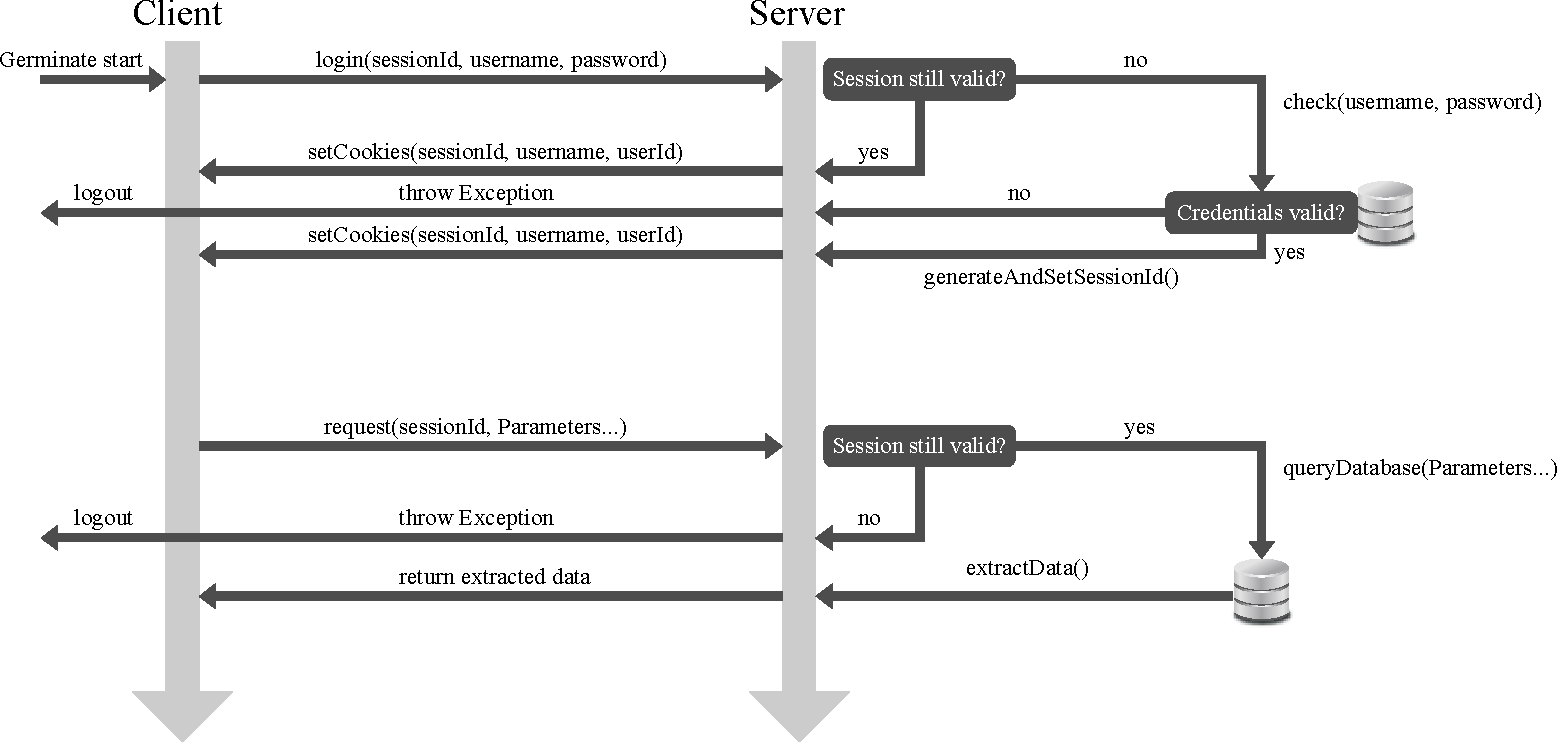
\includegraphics[scale=0.5]{img/examples/authentication.pdf}
    \caption{Authentication procedure of {\germinate}}
    \label{fig:authentication}
\end{figure}

Figure \ref{fig:authentication} shows the authentication process of {\germinate}. The figure contains two major parts. The upper part visualizes the login process, which is initialized by the user entering his/her credentials. These are sent to the server alongside any session id that is still stored in the client from previous sessions. The server will then check the session id that is received. If the id is still valid, the server will store the session id and return it to the client, which, in turn, will create a cookie containing this id.

If the session id is invalid, the server will check if the username password combination is genuine. This is done by encrypting the password and checking it against the entry in the database. If this check fails, the user will be logged out. Otherwise, the server will create a new session id, store it in the HTTP session and return it to the client, which will create a new cookie using this id. The login process is now complete and both the server (via HTTP session) and the client (via cookie) know the current session id.

For each new request that is made from the client, it will need to send the session id as the payload, \ie each remote procedure call (RPC) has to request the session id as a parameter to ensure the security of the communication. As a consequence if this, the server will receive the session id three times per request, namely via the HTTP session, via the cookie and via the payload. If all of these ids match up, the server can fulfil the client's request and return the data. However, if it fails, the user will be logged out.

As a final remark: Even if you currently do not want to enable the security feature, you should still write your code in a way that ensures it will work properly even when the security feature is enabled. Otherwise you might end up with a security leak.